\documentclass[11pt]{article}
\usepackage[a4paper,margin=2.3cm]{geometry}
\usepackage[T1]{fontenc}
\usepackage{lmodern}
\usepackage{amsmath,amssymb,amsthm}
\usepackage{booktabs,multirow,graphicx}
\usepackage{algorithm}
\usepackage[noend]{algpseudocode}
\usepackage[numbers,sort&compress]{natbib}
\usepackage[hidelinks]{hyperref}
\usepackage{xcolor}
\usepackage{placeins}

\newtheorem{proposition}{Proposition}
\renewcommand{\arraystretch}{1.1}

\title{Constraint-Aware Hierarchical Risk Parity\\for Robust Portfolio Allocation}
\author{Pramukh Rajendra Jain\\
\small School of Computer Science and Engineering, Vellore Institute of Technology, Chennai, India\\
\small \texttt{pramukhjain.9966@gmail.com}}
\date{November 2026}

\begin{document}
\maketitle

\begin{abstract}
Hierarchical Risk Parity (HRP) is a popular portfolio construction method that allocates
capital through a correlation tree instead of inverting a covariance matrix, which makes it
robust to estimation error. However, HRP cannot respect the constraints that real mandates
impose: per-asset limits, sector or asset-class caps and floors, and turnover budgets. We
propose Constraint-Aware HRP (CA-HRP), which keeps HRP's hierarchical risk allocation as a
target and maps it to the feasible portfolio with minimum ex-ante tracking error to it. We
prove that this projection is unique, leaves compliant HRP portfolios unchanged, and
redistributes excess weight as a covariance-based hedge. We also introduce a solver-free
capacity-aware bisection and prove that it always meets per-asset bounds exactly. In a
walk-forward study on 20 multi-asset ETFs (2008--2026), 43 NIFTY~50 stocks (2011--2026)
and 47 US large caps (2006--2026), with the design chosen on a validation period and a
held-out test period, CA-HRP satisfies every constraint at every rebalance, whereas HRP
breaches them at up to 100\% of rebalances and the common clip-and-renormalise fix at up to
46\%. Where constraints bind, CA-HRP raises the Sharpe ratio from 0.76 to 0.91 relative to
Euclidean projection, with 25\% lower volatility and smaller drawdowns, and is competitive
with constrained minimum variance while producing more stable weights. Where constraints
rarely bind, it matches HRP. An ablation shows that the risk-aware projection metric, not
the choice of estimator or clustering rule, drives the gains.

\medskip\noindent\textbf{Keywords:} hierarchical risk parity, portfolio optimisation,
constrained allocation, tracking error, robust estimation, convex optimisation.
\end{abstract}

\section{Introduction}\label{sec:intro}

Mean--variance optimisation \citep{markowitz1952} is the textbook answer to portfolio
construction, yet in practice its outputs are notoriously unstable: small errors in
estimated means and covariances are amplified by the inversion of an ill-conditioned
covariance matrix into extreme, concentrated and rapidly changing weights
\citep{michaud1989,chopra1993}. Out of sample, optimised portfolios frequently fail to beat
naive equal weighting \citep{demiguel2009}. Two families of remedies have emerged. The first
regularises the inputs, for example by shrinking the covariance matrix
\citep{ledoit2004} or by imposing weight constraints, which \citet{jagannathan2003} show
act as a form of shrinkage. The second abandons optimisation altogether in favour of
heuristic risk allocation, such as equal risk contribution \citep{maillard2010}.

Hierarchical Risk Parity (HRP), introduced by \citet{lopezdeprado2016}, belongs to the
second family and has become one of the most popular allocation methods among
practitioners and in open-source libraries. HRP clusters assets by correlation, orders them
so that similar assets are adjacent, and allocates capital top-down by recursively splitting
each cluster in inverse proportion to its risk. Because it never inverts the covariance
matrix, HRP is robust to estimation noise and can handle singular covariance matrices.

HRP has, however, a practical blind spot: it cannot respect constraints. Real mandates
impose per-asset limits (UCITS concentration rules, single-stock caps), sector or
asset-class caps and floors (investment policy statements), and turnover budgets (to control
trading costs). Recursive bisection has no mechanism for any of these, and in our
multi-asset universe unconstrained HRP places on average 86\% of capital in a single
short-term bond fund, breaching a 15\% single-fund cap and a 40\% asset-class cap at
\emph{every} rebalance. The usual fixes are ad hoc: weights are clipped and renormalised,
which can cycle without ever reaching the feasible set, or projected onto it with a
Euclidean distance that ignores how assets co-move.

This paper proposes \textbf{Constraint-Aware Hierarchical Risk Parity (CA-HRP)}, a
principled way to keep HRP's risk allocation while satisfying any set of linear
constraints exactly. Our contributions are:
\begin{enumerate}
\item \textbf{Capacity-aware recursive bisection.} We define a capacity interval for every
node of the HRP tree and clip each split into it. We prove that the interval is never
empty and that per-asset bounds are met exactly, with no solver
(Proposition~\ref{prop:box}). This yields a solver-free variant, CA-HRP-B.
\item \textbf{Tracking-error projection.} We map the HRP target to the feasible portfolio
with minimum ex-ante tracking error to it. We show the projection is unique, leaves
compliant HRP portfolios unchanged, and redistributes excess weight as a covariance-based
hedge rather than uniformly (Proposition~\ref{prop:te}).
\item \textbf{A transparent evaluation protocol.} The method design was selected on a
validation period only and then frozen; we report a separate held-out test period, all
constraint sets were fixed before any backtest was run, and all code and data are public.
\item \textbf{Evidence on six universes and in simulation.} On 20 multi-asset ETFs
(2008--2026), 43 NIFTY~50 stocks (2011--2026) and 47 US large caps (2006--2026), and on three
external-validation universes added after the method was frozen (Indian ETFs, US sector
funds and global country funds), CA-HRP satisfies every constraint at every rebalance and at
every rebalancing frequency. Where constraints bind, it is the strongest member of the HRP
family; where they rarely bind, it matches HRP. In a Monte Carlo study with a known
covariance it has the highest true Sharpe ratio of all methods.
\item \textbf{A regime-robust variant and two negative results.} We propose a worst-case
tracking-error projection over covariance scenarios with a guarantee over their convex hull
(Proposition~\ref{prop:robust}), and report honestly that it does not improve on CA-HRP,
and that embedding constraints inside the bisection performs worse than projecting
afterwards.
\end{enumerate}

The rest of the paper is organised as follows. Section~\ref{sec:related} reviews related
work, Section~\ref{sec:setting} states the problem, Section~\ref{sec:method} presents the
method and its properties, Section~\ref{sec:design} describes the data and experimental
protocol, Section~\ref{sec:results} reports the main results, Section~\ref{sec:extended}
the extended evaluation, and Section~\ref{sec:conclusion} concludes.

\section{Related Work}\label{sec:related}

\paragraph{Estimation error and robust allocation.} The sensitivity of mean--variance
portfolios to input error is well documented \citep{michaud1989,chopra1993}.
\citet{demiguel2009} find that across many data sets none of fourteen optimised models
consistently beats $1/N$ out of sample. Shrinkage estimators \citep{ledoit2004} reduce the
condition number of the covariance matrix, and \citet{jagannathan2003} show that
no-short-sale constraints behave like covariance shrinkage. Risk-based methods allocate by
risk rather than expected return; the equal-risk-contribution (ERC) portfolio
\citep{maillard2010} equalises marginal risk contributions and can be computed by convex
optimisation \citep{spinu2013}.

\paragraph{Hierarchical allocation.} \citet{lopezdeprado2016} introduced HRP, combining
graph-theoretic clustering with recursive inverse-variance bisection. \citet{raffinot2017}
studied hierarchical clustering-based allocation more broadly, and \citet{raffinot2018}
proposed the Hierarchical Equal Risk Contribution (HERC) portfolio, which splits along the
dendrogram rather than the ordered list. \citet{pfitzinger2019} recognised that HRP lacks
constraint handling and proposed a cluster-based capital allocation that accommodates
weight bounds within the bisection.

\paragraph{Positioning of this work.} Capacity-aware bisection is closest in spirit to
\citet{pfitzinger2019}; our contribution is a capacity definition that also incorporates
group caps, together with a short proof of non-emptiness and exact box feasibility based on
the additivity and sub-additivity of the capacity bounds. More importantly, we show
empirically that enforcing constraints \emph{inside} the bisection has a hidden cost: excess
weight cascades down one branch and can concentrate in volatile assets. Our main method
therefore separates the two concerns: HRP supplies the risk allocation, and a
tracking-error projection \citep{roll1992} enforces arbitrary linear constraints
(group floors, caps and turnover) with minimum risk distortion. To our knowledge this is
the first study to compare constraint-handling strategies for HRP under a common,
pre-registered protocol with a held-out test period.

\section{Problem Setting}\label{sec:setting}

We consider $N$ risky assets with daily simple returns $r_t\in\mathbb{R}^N$. At each
rebalancing date the manager observes the last $L$ return vectors, estimates a covariance
matrix $\hat\Sigma$, and chooses weights $w\in\mathbb{R}^N$. The mandate imposes a
polyhedral feasible set
\begin{equation}\label{eq:feasible}
\mathcal{W}(w^-)=\Bigl\{w:\ \mathbf{1}^\top w=1,\ \ \ell\le w\le u,\ \
\underline{c}_g\le \sum_{i\in g} w_i\le \bar c_g\ \ \forall g\in\mathcal{G},\ \
\lVert w-w^-\rVert_1\le\tau\Bigr\},
\end{equation}
where $\ell,u$ are per-asset bounds, $\mathcal{G}$ partitions the assets into groups
(sectors or asset classes) with caps $\bar c_g$ and floors $\underline{c}_g$, $w^-$ is the
drifted pre-trade portfolio and $\tau$ a turnover budget. All constraints are linear, so
$\mathcal{W}$ is a convex polytope. We assume it is non-empty. The turnover budget can in
principle conflict with the other constraints if price drift pushes the pre-trade
portfolio far outside the box or group limits; our implementation then relaxes the
turnover cap for that date only. In all experiments reported here this fallback was never
triggered: every CA-HRP portfolio satisfied all constraints, turnover included.

\section{Method}\label{sec:method}

\subsection{Hierarchical Risk Parity}
HRP \citep{lopezdeprado2016} proceeds in three steps. (i)~\emph{Tree clustering}: the
correlation matrix $\rho$ implied by $\hat\Sigma$ is mapped to the distance
$d_{ij}=\sqrt{(1-\rho_{ij})/2}$ and agglomerated with single linkage. (ii)~\emph{Quasi-
diagonalisation}: assets are ordered by the dendrogram leaves so that similar assets are
adjacent. (iii)~\emph{Recursive bisection}: starting from the full ordered list with weight
$W=1$, every cluster $C$ is split into a left and right half $C_L,C_R$; with
$V_S=\tilde w_S^\top\hat\Sigma_{SS}\tilde w_S$ the variance of the inverse-variance portfolio
$\tilde w_S\propto\operatorname{diag}(\hat\Sigma_{SS})^{-1}$ of a cluster $S$, the split
fraction is
\begin{equation}\label{eq:alpha}
\alpha_C = 1-\frac{V_{C_L}}{V_{C_L}+V_{C_R}},\qquad
W_{C_L}=\alpha_C W_C,\quad W_{C_R}=(1-\alpha_C)W_C .
\end{equation}
The recursion ends at single assets. No matrix is inverted and every split is a
two-asset risk-parity decision, which is the source of HRP's stability. Nothing in
\eqref{eq:alpha}, however, knows about $\mathcal{W}$.

\subsection{Capacity-aware recursive bisection (CA-HRP-B)}
Our first contribution makes the bisection itself respect per-asset bounds and, partially,
group caps, without any optimisation solver. For a set of assets $S$ define its
\emph{capacity interval}
\begin{equation}\label{eq:capacity}
\mathrm{lo}(S)=\sum_{i\in S}\ell_i,\qquad
\mathrm{hi}(S)=\sum_{g\in\mathcal{G}}\min\Bigl(\sum_{i\in S\cap g}u_i,\ \bar c_g\Bigr).
\end{equation}
$\mathrm{lo}(S)$ is the least weight that $S$ must hold and $\mathrm{hi}(S)$ an upper
bound on what it can hold. When a cluster $C$ carrying weight $W_C$ is split, the HRP
fraction \eqref{eq:alpha} is clipped to
\begin{equation}\label{eq:clip}
\alpha_C\in\Bigl[\tfrac{\max(\mathrm{lo}(C_L),\,W_C-\mathrm{hi}(C_R))}{W_C},\ \
\tfrac{\min(\mathrm{hi}(C_L),\,W_C-\mathrm{lo}(C_R))}{W_C}\Bigr].
\end{equation}

\begin{proposition}[Exact box feasibility]\label{prop:box}
If $\mathrm{lo}(\{1,\dots,N\})\le 1\le \mathrm{hi}(\{1,\dots,N\})$, the interval
\eqref{eq:clip} is non-empty at every split, and the resulting weights satisfy
$\mathbf{1}^\top w=1$ and $\ell_i\le w_i\le\min(u_i,\bar c_{g(i)})$ for all $i$.
\end{proposition}
\begin{proof}
We show by induction that every cluster satisfies the invariant
$\mathrm{lo}(C)\le W_C\le \mathrm{hi}(C)$. It holds at the root by assumption. Note that
$\mathrm{lo}$ is additive, $\mathrm{lo}(C)=\mathrm{lo}(C_L)+\mathrm{lo}(C_R)$, and
$\mathrm{hi}$ is sub-additive because $\min(a+b,c)\le\min(a,c)+\min(b,c)$ for
$a,b,c\ge0$, so $\mathrm{hi}(C)\le\mathrm{hi}(C_L)+\mathrm{hi}(C_R)$. The interval
\eqref{eq:clip} (multiplied by $W_C$) is non-empty iff the four inequalities
$\mathrm{lo}(C_L)\le\mathrm{hi}(C_L)$, $\mathrm{lo}(C_L)\le W_C-\mathrm{lo}(C_R)$,
$W_C-\mathrm{hi}(C_R)\le\mathrm{hi}(C_L)$ and $W_C-\mathrm{hi}(C_R)\le W_C-\mathrm{lo}(C_R)$
hold. The first and last follow from $\ell\le u$; the second from
$W_C\ge\mathrm{lo}(C)$ and additivity; the third from $W_C\le\mathrm{hi}(C)$ and
sub-additivity. Any $\alpha_C$ in the interval gives children with
$\mathrm{lo}(C_L)\le W_{C_L}\le\mathrm{hi}(C_L)$ and likewise for $C_R$, which preserves
the invariant. At a leaf $\{i\}$, $\mathrm{lo}=\ell_i$ and $\mathrm{hi}=\min(u_i,\bar
c_{g(i)})$, which proves the claim. Weights sum to one because each split conserves
$W_C$.
\end{proof}

CA-HRP-B costs $O(N^2)$ beyond HRP and needs no solver. It guarantees box bounds exactly,
but group constraints are only respected when a group lies inside one sub-tree, and group
floors and turnover are not handled. Those remaining constraints are enforced by a light
projection (next subsection, with the Euclidean metric replaced by a tree-weighted one;
details in the code). As our experiments show, the price of handling constraints
\emph{inside} the bisection is that excess weight cascades down a single branch of the
tree and can end up concentrated in volatile assets; this motivates the main method.

\subsection{Tracking-error projection (CA-HRP)}
The key observation is that HRP produces an excellent \emph{target} but has no notion of
distance between portfolios. Practitioners close the gap by clipping and renormalising,
which is not guaranteed to reach $\mathcal{W}$, or by a Euclidean projection
$\min_{w\in\mathcal{W}}\lVert w-w^{\mathrm{HRP}}\rVert_2^2$, which treats a unit of weight
moved from a short-term bond fund to an oil fund the same as one moved to another bond fund.
We instead measure distance in \emph{risk}: the ex-ante tracking-error variance of the
constrained portfolio relative to HRP \citep{roll1992},
\begin{equation}\label{eq:te}
w^{\mathrm{CA}}=\arg\min_{w\in\mathcal{W}(w^-)}\ (w-w^{\mathrm{HRP}})^\top\,\bar\Sigma\,
(w-w^{\mathrm{HRP}}),\qquad
\bar\Sigma=\frac{N\hat\Sigma_{\mathrm{LW}}}{\operatorname{tr}\hat\Sigma_{\mathrm{LW}}}+\epsilon I,
\end{equation}
where $\hat\Sigma_{\mathrm{LW}}$ is the Ledoit--Wolf shrinkage estimator
\citep{ledoit2004}, $w^{\mathrm{HRP}}$ is HRP computed on $\hat\Sigma_{\mathrm{LW}}$, and
the small ridge $\epsilon=10^{-4}$ guarantees strict convexity.

\begin{proposition}[Properties of the projection]\label{prop:te}
(a) If $\mathcal{W}(w^-)\neq\emptyset$, problem \eqref{eq:te} has a unique solution.
(b) If $w^{\mathrm{HRP}}\in\mathcal{W}(w^-)$ then $w^{\mathrm{CA}}=w^{\mathrm{HRP}}$:
CA-HRP never alters HRP when HRP already complies.
(c) Among all feasible portfolios, $w^{\mathrm{CA}}$ minimises the ex-ante variance of
the return difference to HRP, so it is the feasible portfolio whose returns are most
correlated with, and least volatile around, the HRP portfolio.
(d) Let $A w\le b$ collect the active inequality constraints and $\mathbf 1^\top w=1$ the
budget. The KKT conditions give
$w^{\mathrm{CA}}=w^{\mathrm{HRP}}-\tfrac12\bar\Sigma^{-1}(A^\top\lambda+\nu\mathbf{1})$
with $\lambda\ge0$: the correction is a \emph{hedge}. Weight removed from a capped
asset is redistributed in proportion to the rows of $\bar\Sigma^{-1}$, i.e.\ towards the
assets that best replicate the capped asset's risk.
\end{proposition}
\begin{proof}
(a) $\bar\Sigma\succ0$, so the objective is strictly convex and $\mathcal{W}$ is a non-empty
closed convex set; a unique minimiser exists. (b) The objective is non-negative and zero at
$w^{\mathrm{HRP}}$. (c) $(w-w^{\mathrm{HRP}})^\top\hat\Sigma(w-w^{\mathrm{HRP}})$ is the
variance of $(w-w^{\mathrm{HRP}})^\top r$ under the estimated covariance; the trace
normalisation and ridge only rescale and regularise it. (d) Stationarity of the
Lagrangian $(w-w^{\mathrm{HRP}})^\top\bar\Sigma(w-w^{\mathrm{HRP}})+\lambda^\top(Aw-b)
+\nu(\mathbf{1}^\top w-1)$, with the $\ell_1$ turnover constraint written in its standard
linear epigraph form.
\end{proof}

Part (d) explains the behaviour we observe in the multi-asset universe: when HRP wants far
more than the 40\% asset-class cap in bonds, the Euclidean projection spreads the excess
almost uniformly (about 5\% to each non-bond fund), while the tracking-error projection
re-shapes the portfolio as a hedge: inside the bond budget it moves from short-term to
intermediate and long Treasuries (IEF, TLT), whose negative correlation with equities
offsets the risk of the assets that must now be held, and outside the bond budget it
favours gold and broad commodities (Section~\ref{sec:results}). The constrained portfolio
keeps the defensive character of HRP, with markedly lower volatility than the Euclidean
alternative.

\begin{algorithm}[t]
\caption{Constraint-Aware HRP (one rebalancing date)}\label{alg:cahrp}
\begin{algorithmic}[1]
\Require returns window $R\in\mathbb{R}^{L\times N}$, feasible set $\mathcal{W}$, drifted weights $w^-$
\State $\hat\Sigma_{\mathrm{LW}}\gets$ Ledoit--Wolf shrinkage covariance of $R$
\State $\rho\gets$ correlation of $\hat\Sigma_{\mathrm{LW}}$;\ \ $d_{ij}\gets\sqrt{(1-\rho_{ij})/2}$
\State $\pi\gets$ leaf order of the single-linkage dendrogram of $d$
\State $w^{\mathrm{HRP}}\gets$ recursive bisection \eqref{eq:alpha} on $\pi$
\Comment{optionally clipped by \eqref{eq:clip}}
\State $w^{\mathrm{CA}}\gets$ solve the convex QP \eqref{eq:te} over $\mathcal{W}(w^-)$
\State \Return $w^{\mathrm{CA}}$
\end{algorithmic}
\end{algorithm}

\paragraph{Complexity.} Steps 1--4 cost $O(LN^2+N^2\log N)$. Step~5 is a QP with $N$
variables (plus $N$ auxiliary variables for the turnover epigraph) and $N+|\mathcal{G}|$
linear constraints; with an interior-point solver \citep{diamond2016} it takes a few
milliseconds for $N\le 50$. A full 20-year monthly backtest of CA-HRP runs in under
six seconds on a laptop; Section~\ref{sec:extended} reports timings up to $N=400$.

\subsection{Two further properties: noise damping and the price of compliance}
\label{sec:props}

\begin{proposition}[Noise damping]\label{prop:nonexp}
Fix the metric $\bar\Sigma\succ0$ and the feasible set $\mathcal{W}$, and let
$P(t)=\arg\min_{w\in\mathcal{W}}\lVert w-t\rVert_{\bar\Sigma}$ with
$\lVert x\rVert_{\bar\Sigma}^2=x^\top\bar\Sigma x$. Then for any two targets $t_1,t_2$,
$\lVert P(t_1)-P(t_2)\rVert_{\bar\Sigma}\le\lVert t_1-t_2\rVert_{\bar\Sigma}$.
\end{proposition}
\begin{proof}
$\langle x,y\rangle_{\bar\Sigma}=x^\top\bar\Sigma y$ is an inner product, so $P$ is the
metric projection onto a closed convex set in a Hilbert space, which is firmly
non-expansive \citep{bauschke2017}: $\lVert P t_1-Pt_2\rVert^2\le\langle Pt_1-Pt_2,\,t_1-t_2\rangle\le
\lVert Pt_1-Pt_2\rVert\,\lVert t_1-t_2\rVert$ by the variational inequality characterising
projections and the Cauchy--Schwarz inequality.
\end{proof}

Proposition~\ref{prop:nonexp} means that whatever estimation noise the HRP target carries,
the projection can only shrink it, measured in the same risk metric. The clip-and-renormalise
heuristic has no such property; Section~\ref{sec:round3} shows that in practice it often
\emph{amplifies} noise.

\begin{proposition}[Exact price-of-compliance identity]\label{prop:kkt}
Let $f^\star=(w^{\mathrm{CA}}-t)^\top\bar\Sigma(w^{\mathrm{CA}}-t)$ be the optimal value of
\eqref{eq:te} with linear constraints $a_k^\top w\le b_k$ and multipliers
$\lambda_k\ge0$. Then
\begin{equation}\label{eq:kkt}
f^\star=\tfrac12\sum_k\lambda_k\,(a_k^\top t-b_k),
\end{equation}
so the cost of compliance splits exactly over constraints, each term being the shadow price
of a constraint times the amount by which the HRP target $t$ violates it.
\end{proposition}
\begin{proof}
Stationarity gives $2\bar\Sigma d=-(\sum_k\lambda_k a_k+\nu\mathbf1)$ with $d=w^{\mathrm{CA}}-t$.
Multiply by $d^\top/2$: $f^\star=-\tfrac12\sum_k\lambda_k a_k^\top d$, because
$\mathbf1^\top d=0$. Complementary slackness gives
\[
\lambda_k a_k^\top w^{\mathrm{CA}}=\lambda_k b_k,\qquad\text{hence}\qquad
-\lambda_k a_k^\top d=\lambda_k(a_k^\top t-b_k).
\]
\end{proof}

Individual terms of \eqref{eq:kkt} can be negative: a cap that the target already satisfies
but that binds at the optimum contributes negatively. To report the cost by \emph{family} of
constraints (asset caps; group caps and floors; turnover) we therefore use the Shapley value \citep{shapley1953}
of the cooperative game $v(S)=f^\star_S$, the optimal value when only the families in $S$
are imposed. It is order-independent and adds up exactly to $f^\star$, and it costs $2^3=8$
small solves per date. The $\ell_1$ turnover cap is not linear in $w$, but in its standard
linear epigraph form the identity still holds; we compute the turnover term as
$f^\star$ minus the linear terms and use \eqref{eq:kkt} as an exactness check on every date
(the remainder must vanish whenever the turnover cap is slack).

\subsection{Regime-robust projection (CA-HRP-R)}\label{sec:robust}
The tracking-error metric in \eqref{eq:te} trusts a single covariance estimate. When
correlations shift, the hedge chosen by the projection can fail. We therefore also study a
\emph{regime-robust} projection that tracks HRP under the worst of $K$ covariance
scenarios $\{\Sigma_k\}_{k=1}^K$:
\begin{equation}\label{eq:robust}
w^{\mathrm{R}}=\arg\min_{w\in\mathcal{W}(w^-)}\ \max_{k=1,\dots,K}\
(w-w^{\mathrm{HRP}})^\top\bar\Sigma_k(w-w^{\mathrm{HRP}}),
\end{equation}
where every $\bar\Sigma_k$ uses the same scale factor as the baseline estimate, so that
relative risk levels across regimes are preserved. We consider three scenarios: the
1-year Ledoit--Wolf estimate, a 3-month (63-day) Ledoit--Wolf estimate capturing the
current regime, and a ``hedges-fail'' stress covariance
$D\lvert\rho\rvert D$ in which every correlation is replaced by its absolute value.

\begin{proposition}[Robust projection]\label{prop:robust}
Problem \eqref{eq:robust} is convex, has a unique solution, and returns $w^{\mathrm{HRP}}$
whenever it is feasible. Its optimal value $t^\star$ bounds the ex-ante tracking-error
variance under \emph{every} covariance matrix in the convex hull
$\operatorname{conv}\{\bar\Sigma_1,\dots,\bar\Sigma_K\}$:
$(w^{\mathrm{R}}-w^{\mathrm{HRP}})^\top\Sigma(w^{\mathrm{R}}-w^{\mathrm{HRP}})\le t^\star$.
\end{proposition}
\begin{proof}
Each term is a strictly convex quadratic, and the pointwise maximum of strictly convex
functions is strictly convex; with a non-empty convex feasible set this gives existence
and uniqueness, and the objective is zero only at $w^{\mathrm{HRP}}$. For
$\Sigma=\sum_k\lambda_k\bar\Sigma_k$ with $\lambda$ in the simplex and $d=w-w^{\mathrm{HRP}}$,
$d^\top\Sigma d=\sum_k\lambda_k d^\top\bar\Sigma_k d\le\max_k d^\top\bar\Sigma_k d$, because
the tracking-error variance is linear in $\Sigma$.
\end{proof}

Problem \eqref{eq:robust} is a second-order cone program (epigraph form) and solves as fast
as \eqref{eq:te}. The choice of scenarios was made on the validation period only
(Appendix~\ref{app:design}): the variant using the 1-year and 3-month regimes was selected.
The hedges-fail stress scenario was rejected at that stage because it lowered validation
performance markedly, even though the held-out period later contained exactly such a
regime (2022). We report the frozen choice regardless.

\section{Experimental Design}\label{sec:design}

\paragraph{Data.} We use daily dividend- and split-adjusted closing prices from Yahoo
Finance for three universes chosen to span different constraint regimes
(Table~\ref{tab:universes}): (i)~20 US-listed multi-asset ETFs covering equities, government
and corporate bonds, commodities and real estate (January 2008 -- October 2026);
(ii)~43 long-listed constituents of India's NIFTY~50 index across 12 sectors
(January 2011 -- October 2026); (iii)~47 US large-cap stocks across 11 sectors
(January 2006 -- October 2026). All series are complete over their sample. Survivorship
bias affects the stock universes, which consist of current large caps; it affects all
methods equally and does not change their ranking, which is our object of study.

\begin{table}[!htbp]
\centering\small
\caption{Universes and constraint sets. Constraint sets were fixed before any backtest.}
\label{tab:universes}
\begin{tabular}{lccc}
\toprule
 & Multi-asset ETFs & NIFTY 50 stocks & US large caps\\
\midrule
Assets / groups & 20 / 4 & 43 / 12 & 47 / 11\\
Sample & 2008--2026 & 2011--2026 & 2006--2026\\
Per-asset cap $u_i$ & 15\% & 6\% & 6\%\\
Group cap $\bar c_g$ & 40\% & 25\% & 20\%\\
Group floor $\underline c_g$ & Equity $\ge$ 20\% & -- & --\\
Turnover budget $\tau$ (per month) & 30\% & 30\% & 30\%\\
Validation / test split & 2016 | 2017-- & 2018 | 2019-- & 2015 | 2016--\\
\bottomrule
\end{tabular}
\end{table}

\paragraph{Constraints.} The constraint sets mirror typical mandates: a single-holding cap
of roughly $2.5/N$, sector or asset-class caps, a growth floor of 20\% in equities for the
multi-asset portfolio, and a monthly two-sided turnover budget of 30\%. All weights are
long-only and fully invested.

\paragraph{Methods compared.} \emph{Unconstrained references}: equal weight (EW),
inverse variance (IVP), long-only minimum variance (MinVar), equal risk contribution (ERC)
and standard HRP. \emph{Constrained competitors}: minimum variance (MinVar-C) and
mean--variance with risk aversion 5 (MVO-C), both solved over the full feasible set;
HRP with iterative clipping and renormalisation (HRP-Clip, the common practitioner fix,
which ignores turnover); and HRP followed by Euclidean projection onto the full feasible set
(HRP-Proj). \emph{Proposed}: the solver-free capacity-aware bisection (CA-HRP-B) and the
full method with tracking-error projection (CA-HRP). Covariance-based competitors use the
Ledoit--Wolf estimator, except the HRP baselines, which follow the original sample-covariance
recipe.

\paragraph{Backtest protocol.} At each month end we estimate inputs from the previous
$L=252$ trading days, compute target weights, and trade at the close. Between rebalances
weights drift with prices. Turnover is $\lVert w_t-w_t^-\rVert_1$ against the drifted
weights, and a cost of 10\,bps per unit of turnover is deducted (we also report 0, 25 and
50\,bps). Constraint compliance is checked on the target weights at every rebalance.

\paragraph{Design selection and held-out test.} An initial version of CA-HRP enforced
all constraints inside the bisection followed by a tree-weighted projection. Before
finalising the method, we compared eight configurations \emph{on the validation period
only} (first part of each sample, Table~\ref{tab:universes}) and selected the
tracking-error projection with Ledoit--Wolf covariance (Appendix~\ref{app:design}). The
configuration was then frozen, and we report results both over the full sample and over the
untouched test period.

\paragraph{Metrics.} Annualised return (CAGR), volatility, Sharpe ratio (zero risk-free
rate), maximum drawdown, daily 5\% CVaR, annualised turnover, constraint-violation rate
(share of rebalances with any breach), realised tracking error to unconstrained HRP
(TE$_{\text{HRP}}$), effective number of holdings $1/\sum_i w_i^2$, and risk concentration,
the Herfindahl index of percentage risk contributions scaled by $N$ (1 = equal risk). Sharpe
ratio differences are tested with a circular block bootstrap (block of 21 days, 2{,}000
replications) in the spirit of \citet{ledoit2008} and \citet{politis1994}.

\FloatBarrier
\section{Results}\label{sec:results}

\begin{table*}[!htbp]\centering\small
\caption{Full-sample out-of-sample results, net of 10\,bps costs. CAGR, Vol, MaxDD, CVaR and TE$_{\text{HRP}}$ in \%; turnover annualised; Viol = share of rebalances breaching any constraint; $p$ = bootstrap $p$-value of the Sharpe difference with CA-HRP. Unconstrained methods (top block) are shown for reference only. Best constrained Sharpe ratio in bold.}\label{tab:main}
\setlength{\tabcolsep}{4.5pt}\begin{tabular}{llrrrrrrrrrr}\toprule
Universe & Method & CAGR & Vol & Sharpe & $p$ & MaxDD & CVaR$_{5}$ & Turn. & Viol & TE$_{\text{HRP}}$ & Eff.\,N\\\midrule
\multirow{11}{*}{\rotatebox{90}{Multi-asset ETFs}} & EW & 8.0 & 10.9 & 0.763 & 0.12 & -24.8 & -1.63 & 0.34 & 0\% & 10.2 & 20.0\\
 & IVP & 1.9 & 2.2 & 0.840 & 0.70 & -9.6 & -0.34 & 0.30 & 100\% & 0.5 & 1.6\\
 & MinVar & 2.4 & 2.4 & 0.971 & 0.68 & -9.1 & -0.36 & 0.90 & 100\% & 1.4 & 2.5\\
 & ERC & 4.8 & 5.7 & 0.852 & 0.47 & -17.3 & -0.84 & 0.48 & 100\% & 4.5 & 9.3\\
 & HRP & 1.6 & 2.0 & 0.833 & 0.70 & -8.8 & -0.30 & 0.63 & 100\% & 0.0 & 1.4\\
\cmidrule{2-12}
 & MinVar-C & 6.8 & 7.3 & \textbf{0.935} & 0.34 & -17.5 & -1.07 & 1.21 & 0\% & 6.5 & 8.0\\
 & MVO-C & 8.8 & 12.2 & 0.753 & 0.30 & -19.1 & -1.91 & 3.16 & 0\% & 11.6 & 7.3\\
 & HRP-Clip & 6.3 & 9.2 & 0.709 & 0.01 & -22.8 & -1.37 & 2.17 & 46\% & 8.4 & 13.9\\
 & HRP-Proj & 7.4 & 9.9 & 0.764 & 0.13 & -22.8 & -1.49 & 0.62 & 0\% & 9.3 & 16.1\\
 & CA-HRP-B & 7.1 & 9.8 & 0.750 & 0.14 & -21.4 & -1.47 & 2.50 & 0\% & 9.2 & 10.7\\
 & \textbf{CA-HRP} & 6.6 & 7.4 & 0.908 & -- & -18.8 & -1.08 & 1.25 & 0\% & 6.4 & 8.3\\
\midrule
\multirow{11}{*}{\rotatebox{90}{NIFTY 50 stocks}} & EW & 19.7 & 15.4 & 1.247 & 0.07 & -36.0 & -2.21 & 0.62 & 0\% & 3.7 & 43.0\\
 & IVP & 18.7 & 14.3 & 1.272 & 0.02 & -33.4 & -2.04 & 0.85 & 17\% & 2.0 & 37.8\\
 & MinVar & 18.0 & 12.8 & 1.356 & 0.89 & -26.1 & -1.74 & 2.87 & 100\% & 4.7 & 14.1\\
 & ERC & 19.5 & 14.2 & 1.326 & 0.22 & -32.7 & -2.02 & 0.81 & 3\% & 1.8 & 39.0\\
 & HRP & 19.5 & 13.7 & 1.368 & 0.96 & -30.6 & -1.94 & 2.70 & 48\% & 0.0 & 32.4\\
\cmidrule{2-12}
 & MinVar-C & 18.6 & 12.8 & \textbf{1.401} & 0.62 & -26.5 & -1.76 & 2.12 & 0\% & 3.5 & 19.8\\
 & MVO-C & 20.2 & 16.2 & 1.216 & 0.17 & -33.2 & -2.35 & 3.35 & 0\% & 6.8 & 17.4\\
 & HRP-Clip & 19.6 & 13.7 & 1.369 & 1.00 & -30.6 & -1.95 & 2.66 & 8\% & 0.2 & 32.8\\
 & HRP-Proj & 19.6 & 13.8 & 1.368 & 0.97 & -30.6 & -1.95 & 2.62 & 0\% & 0.2 & 32.9\\
 & CA-HRP-B & 19.5 & 13.7 & 1.368 & 0.68 & -30.1 & -1.95 & 2.51 & 0\% & 0.9 & 33.1\\
 & \textbf{CA-HRP} & 19.5 & 13.7 & 1.369 & -- & -30.1 & -1.94 & 2.47 & 0\% & 0.9 & 33.1\\
\midrule
\multirow{11}{*}{\rotatebox{90}{US large caps}} & EW & 13.3 & 18.5 & 0.767 & 0.59 & -47.9 & -2.80 & 0.53 & 0\% & 4.8 & 47.0\\
 & IVP & 11.7 & 16.1 & 0.768 & 0.15 & -41.1 & -2.40 & 0.73 & 24\% & 1.3 & 37.0\\
 & MinVar & 9.3 & 13.7 & 0.720 & 0.39 & -33.0 & -1.98 & 3.02 & 100\% & 6.2 & 10.5\\
 & ERC & 12.4 & 16.8 & 0.781 & 0.67 & -44.7 & -2.54 & 0.68 & 3\% & 2.3 & 42.6\\
 & HRP & 11.6 & 15.7 & 0.776 & 0.14 & -40.7 & -2.35 & 2.88 & 66\% & 0.0 & 33.9\\
\cmidrule{2-12}
 & MinVar-C & 10.7 & 14.5 & 0.773 & 0.66 & -35.7 & -2.15 & 2.06 & 0\% & 3.6 & 19.5\\
 & MVO-C & 12.7 & 17.5 & 0.774 & 0.82 & -43.2 & -2.64 & 3.43 & 0\% & 6.9 & 17.5\\
 & HRP-Clip & 11.6 & 15.8 & 0.775 & 0.12 & -41.1 & -2.37 & 2.80 & 8\% & 0.3 & 34.6\\
 & HRP-Proj & 11.7 & 15.8 & 0.775 & 0.11 & -41.2 & -2.37 & 2.76 & 0\% & 0.3 & 34.7\\
 & CA-HRP-B & 11.9 & 15.8 & 0.790 & 0.55 & -41.9 & -2.36 & 2.65 & 0\% & 1.0 & 34.8\\
 & \textbf{CA-HRP} & 11.9 & 15.7 & \textbf{0.793} & -- & -40.4 & -2.35 & 2.57 & 0\% & 0.9 & 34.7\\
\bottomrule
\end{tabular}\end{table*}

\subsection{Constraint compliance}
Table~\ref{tab:main} first answers the practical question. Unconstrained HRP breaches the
mandate at 100\% of rebalances in the multi-asset universe, 48\% for NIFTY and 66\% for
US stocks. The common practitioner fix, HRP-Clip, still breaches constraints at 46\%, 8\%
and 8\% of rebalances respectively: alternating clipping and group rescaling can cycle
when per-asset and group limits interact, and it ignores turnover entirely. Every
optimisation-based method, including both CA-HRP variants, satisfies all constraints at
every rebalance, and CA-HRP never needed the turnover fallback.

\subsection{Performance where constraints bind}
The multi-asset universe is where constraints bite hardest: HRP would hold on average 86\%
in a single short-term Treasury fund (Figure~\ref{fig:groups}), so the 15\% fund cap, the
40\% asset-class cap and the 20\% equity floor force a very different portfolio. Here the
way the constraints are enforced matters a great deal. CA-HRP reaches a Sharpe ratio of
0.908 with 7.4\% volatility and a $-18.8\%$ maximum drawdown, against 0.764, 9.9\% and
$-22.8\%$ for the Euclidean projection (HRP-Proj) and 0.709 for HRP-Clip. The difference with
HRP-Clip is significant ($p=0.01$); against HRP-Proj and equal weight the $p$-values are
0.13 and 0.12. Among all constrained methods, only constrained minimum variance has a higher
Sharpe ratio (0.935), a difference that is far from significant ($p=0.34$). CA-HRP's
realised tracking error to HRP (6.4\%) is the lowest of the HRP-family methods, as its
construction intends.

The solver-free CA-HRP-B performs like the Euclidean projection (0.750) but with four
times the turnover. Its bisection handles constraints by pushing excess weight down the
tree, so the portfolio concentrates in whichever volatile branch has spare capacity
(commodities, Figure~\ref{fig:groups} and Section~\ref{sec:method}). This is the central
negative finding that motivated the final design: constraints are best enforced
\emph{after} the risk allocation, in a risk metric, not inside the bisection.

\begin{figure}[t]
\centering
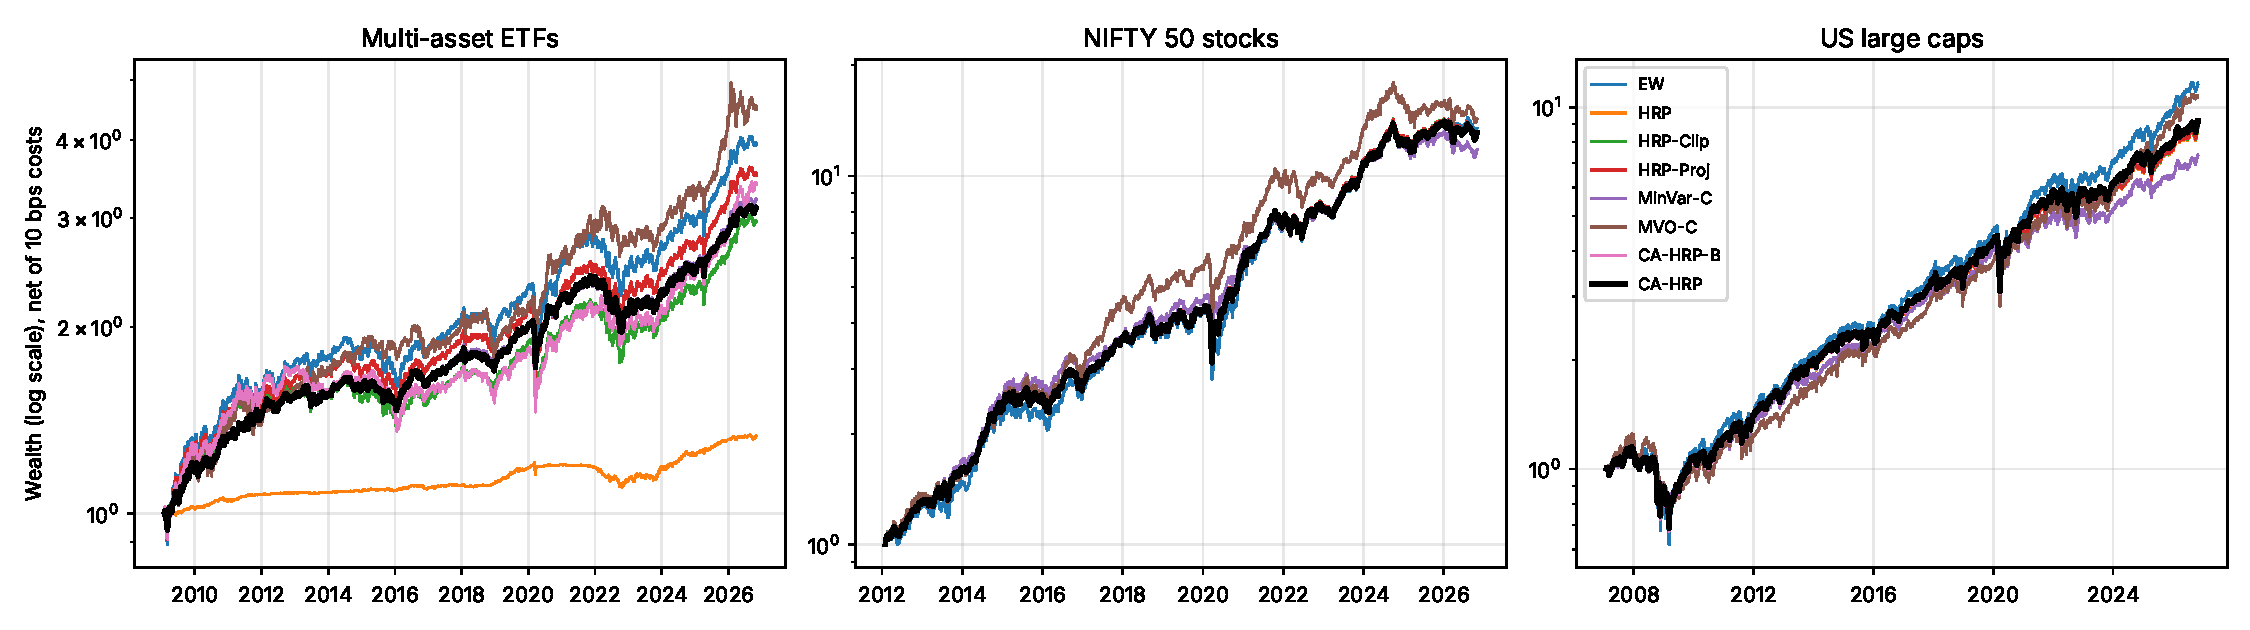
\includegraphics[width=\linewidth]{../results/figures/wealth_curves.pdf}
\caption{Growth of one unit of wealth (log scale), net of 10\,bps costs.}
\label{fig:wealth}
\end{figure}

\begin{figure}[t]
\centering
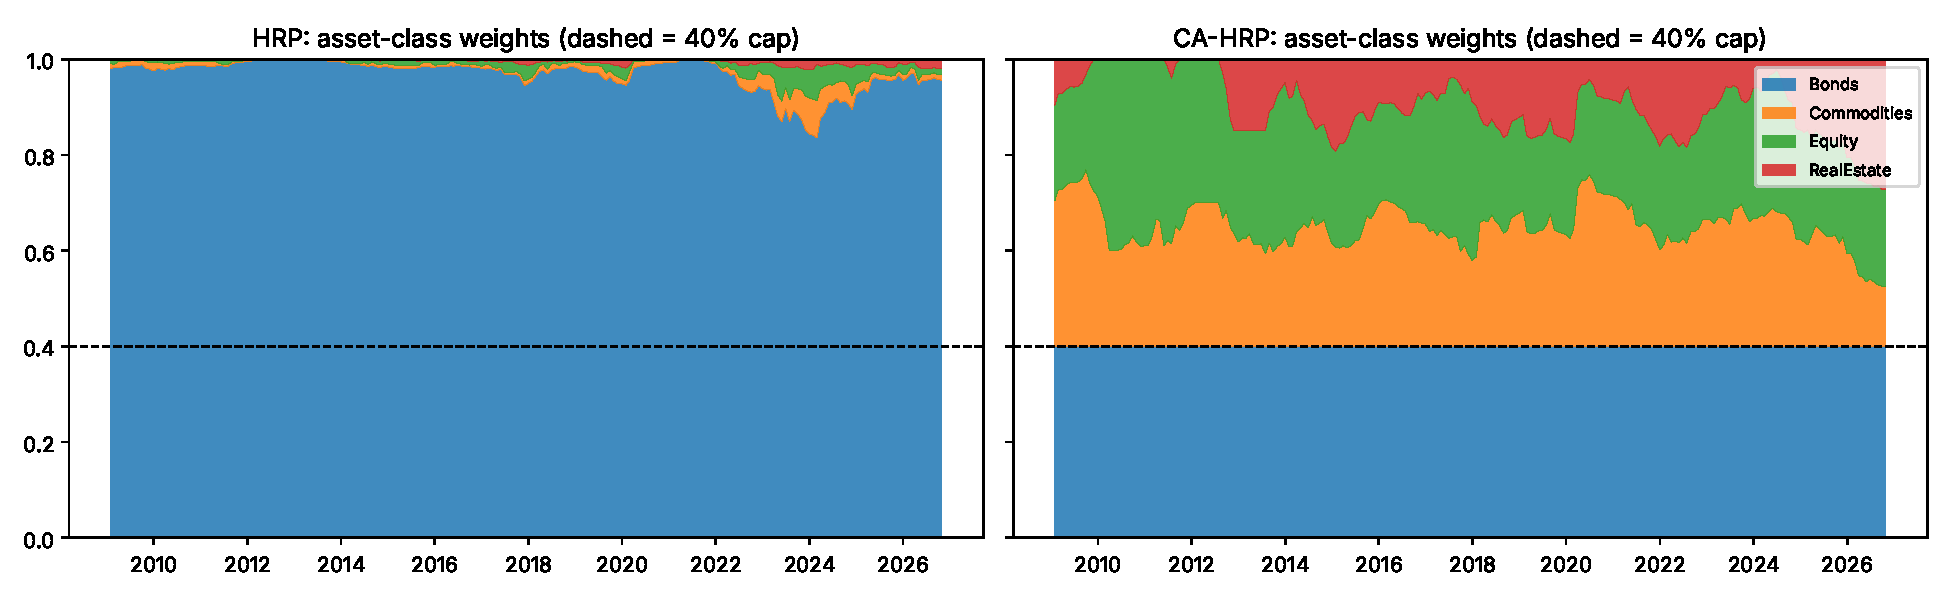
\includegraphics[width=\linewidth]{../results/figures/etf_group_weights.pdf}
\caption{Asset-class weights in the multi-asset universe. Unconstrained HRP (left) is
almost entirely in bonds, far above the 40\% cap. CA-HRP (right) holds bonds at the cap
and allocates the remainder by tracking-error projection.}
\label{fig:groups}
\end{figure}

\subsection{Performance where constraints rarely bind}
In the two stock universes HRP breaches the limits at about half of the rebalances, but only
by small amounts: the realised tracking error between HRP and any of its constrained
versions is at most 1\%. All HRP-based methods are therefore statistically indistinguishable,
which is what Proposition~\ref{prop:te}(b) predicts as the constraints become slack. CA-HRP posts the highest Sharpe ratio
of all eleven methods for US large caps (0.793) and ties HRP for NIFTY (1.369 vs 1.368),
where constrained minimum variance is marginally higher (1.401, $p=0.62$). In other words,
CA-HRP costs nothing when HRP is already compliant and helps when it is not.

\subsection{Held-out test period}
Table~\ref{tab:test} repeats the comparison on the period after the validation window,
which played no role in choosing the design. The ranking is unchanged. In the multi-asset
universe CA-HRP's test Sharpe is 0.929, against 0.805 for HRP-Proj, 0.802 for HRP-Clip,
0.783 for equal weight and 0.977 for constrained minimum variance, with the lowest
volatility of any HRP-family method. In stocks CA-HRP again matches HRP.

\begin{table}[!htbp]\centering\small
\caption{Sharpe ratio (net of 10\,bps) on the held-out test period, which was never used to choose the CA-HRP design, next to the full sample. Vol and MaxDD (\%) on the test period.}\label{tab:test}
\begin{tabular}{l rrr rrr}\toprule
 & \multicolumn{3}{c}{Test-period Sharpe} & \multicolumn{3}{c}{ETFs, test period}\\
\cmidrule(lr){2-4}\cmidrule(lr){5-7}
Method & ETFs & NIFTY & US & Vol & MaxDD & Full-sample SR\\\midrule
EW & 0.783 & 1.066 & 0.972 & 10.6 & -24.8 & 0.763\\
HRP & 0.830 & 1.126 & 0.909 & 2.4 & -8.8 & 0.833\\
MinVar-C & 0.977 & 1.051 & 0.889 & 7.4 & -17.5 & 0.935\\
MVO-C & 0.781 & 0.869 & 0.976 & 12.9 & -19.1 & 0.753\\
HRP-Clip & 0.802 & 1.126 & 0.909 & 8.9 & -22.8 & 0.709\\
HRP-Proj & 0.805 & 1.126 & 0.910 & 9.6 & -22.8 & 0.764\\
CA-HRP-B & 0.876 & 1.122 & 0.947 & 9.5 & -21.3 & 0.750\\
\textbf{CA-HRP} & 0.929 & 1.123 & 0.941 & 7.4 & -18.8 & 0.908\\
\bottomrule\end{tabular}\end{table}

\subsection{Ablation}
Table~\ref{tab:ablation} isolates each design choice. In the multi-asset universe the
\emph{distance metric} drives almost the whole gain: replacing the full-covariance
tracking-error metric by its diagonal lowers the Sharpe ratio from 0.908 to 0.777, and the
Euclidean metric to 0.742. Adding capacity-aware bisection before the projection lowers it
to 0.861 and nearly doubles turnover; adding a tree-consistency penalty has a similar
effect. The choice of covariance estimator, linkage rule and split rule matters little
(Sharpe 0.910--0.922), so the method is not sensitive to those HRP details. Removing the
turnover cap barely changes performance, showing that the cap is rarely binding for CA-HRP
and does not drive its results. In the stock universes no ablation moves the Sharpe ratio
by more than 0.04.

\begin{table}[!htbp]\centering\small
\caption{Ablation of CA-HRP components (full sample, net of 10\,bps). Each row changes one component of the full method.}\label{tab:ablation}
\begin{tabular}{l rrr rrr}\toprule
 & \multicolumn{3}{c}{Sharpe ratio} & \multicolumn{3}{c}{ETFs}\\
\cmidrule(lr){2-4}\cmidrule(lr){5-7}
Variant & ETFs & NIFTY & US & Vol & Turn. & TE$_{\text{HRP}}$\\\midrule
CA-HRP (full) & 0.908 & 1.369 & 0.793 & 7.4 & 1.25 & 6.4\\
\midrule
sample covariance & 0.922 & 1.372 & 0.781 & 7.3 & 1.22 & 6.4\\
diagonal metric & 0.777 & 1.366 & 0.791 & 9.2 & 1.14 & 8.5\\
Euclidean metric & 0.742 & 1.365 & 0.789 & 9.8 & 1.06 & 9.1\\
+ capacity bisection & 0.861 & 1.367 & 0.796 & 8.5 & 2.30 & 7.7\\
+ tree-consistency term & 0.846 & 1.370 & 0.794 & 7.9 & 2.27 & 7.1\\
no turnover cap & 0.910 & 1.369 & 0.793 & 7.3 & 1.26 & 6.4\\
Ward linkage & 0.910 & 1.330 & 0.759 & 7.4 & 1.30 & 6.4\\
dendrogram splits & 0.918 & 1.392 & 0.778 & 7.4 & 1.19 & 6.5\\
\bottomrule\end{tabular}\end{table}

\subsection{Robustness}
\paragraph{Costs and estimation window.} Table~\ref{tab:robust} shows the multi-asset
advantage of CA-HRP over the other HRP-family methods survives 50\,bps costs (0.840 vs 0.739
for HRP-Proj) and both shorter (126-day) and longer (504-day) estimation windows, where
CA-HRP improves on HRP-Proj by 0.14 and 0.19 Sharpe points respectively. Constrained minimum
variance remains a strong competitor throughout.

\paragraph{Stability of weights.} We re-estimate every method on 30 block-bootstrapped
versions of the estimation window at eight dates per universe and measure how much the
weights move. CA-HRP is far more stable than mean--variance (instability 0.16--0.22 vs
0.70--0.78) and more stable than constrained minimum variance in every universe (e.g.\
0.218 vs 0.324 for NIFTY). In the multi-asset universe HRP-Proj is the most stable, because
it is anchored near equal weight; its stability comes at the price of a portfolio that
tracks HRP poorly and has higher volatility.

\begin{table*}[!htbp]\centering\small
\caption{Robustness. Left: Sharpe ratio in the multi-asset universe at 50\,bps costs and with 126- and 504-day estimation windows (all universes). Right: weight instability, the mean $L_1$ distance of bootstrapped weights from their average (lower = more stable).}\label{tab:robust}
\begin{tabular}{l r rrr rrr rrr}\toprule
 & ETFs & \multicolumn{3}{c}{Window 126 days} & \multicolumn{3}{c}{Window 504 days} & \multicolumn{3}{c}{Weight instability}\\
\cmidrule(lr){3-5}\cmidrule(lr){6-8}\cmidrule(lr){9-11}
Method & 50\,bps & ETFs & NIFTY & US & ETFs & NIFTY & US & ETFs & NIFTY & US\\\midrule
EW & 0.750 & 0.535 & 1.197 & 0.794 & 0.701 & 1.196 & 0.775 & -- & -- & --\\
HRP & 0.705 & 0.622 & 1.288 & 0.786 & 0.932 & 1.287 & 0.767 & 0.068 & 0.230 & 0.227\\
MinVar-C & 0.868 & 0.703 & 1.392 & 0.801 & 0.936 & 1.341 & 0.730 & 0.185 & 0.324 & 0.318\\
MVO-C & 0.650 & 0.660 & 1.142 & 0.755 & 0.796 & 1.172 & 0.760 & 0.754 & 0.698 & 0.781\\
HRP-Clip & 0.614 & 0.479 & 1.293 & 0.786 & 0.800 & 1.288 & 0.767 & 0.209 & 0.222 & 0.214\\
HRP-Proj & 0.739 & 0.535 & 1.293 & 0.792 & 0.714 & 1.288 & 0.766 & 0.037 & 0.220 & 0.217\\
\textbf{CA-HRP} & 0.840 & 0.676 & 1.301 & 0.803 & 0.908 & 1.276 & 0.766 & 0.158 & 0.218 & 0.211\\
\bottomrule\end{tabular}\end{table*}

\paragraph{Stress periods.} Table~\ref{tab:stress} reports cumulative returns in three
crises. In the COVID crash CA-HRP lost 6.9\% in the multi-asset universe, against 14.0\% for
HRP-Proj, 13.7\% for HRP-Clip and 14.9\% for equal weight, and it was flat in the GFC window.
The 2022 rates shock is the exception: CA-HRP's hedge tilt towards intermediate and long
Treasuries, which protected it in 2020, lost 17.2\% when bonds and equities fell together,
slightly more than HRP-Proj ($-15.3\%$). This illustrates the main limitation of any
covariance-based hedge: it relies on correlations that can break down.

\begin{table}[!htbp]\centering\small
\caption{Cumulative return (\%) in stress windows: GFC = Sep 2008--Mar 2009, COVID = 15 Feb--30 Apr 2020, Rates = Jan--Oct 2022.}\label{tab:stress}
\setlength{\tabcolsep}{4pt}\begin{tabular}{l rrr r rrr}\toprule
 & \multicolumn{3}{c}{ETFs} & NIFTY & \multicolumn{3}{c}{US}\\
\cmidrule(lr){2-4}\cmidrule(lr){5-5}\cmidrule(lr){6-8}
Method & GFC & COVID & Rates & COVID & GFC & COVID & Rates\\\midrule
EW & -1.6 & -14.9 & -16.9 & -16.8 & -30.4 & -13.5 & -5.1\\
HRP & 0.6 & -0.3 & -6.6 & -9.6 & -24.8 & -10.0 & -5.9\\
MinVar-C & 0.5 & -7.6 & -16.0 & -4.4 & -20.3 & -10.7 & -4.4\\
MVO-C & 0.8 & -4.5 & -8.2 & -13.8 & -30.1 & -9.3 & -0.9\\
HRP-Clip & 0.4 & -13.7 & -17.4 & -9.6 & -24.8 & -10.0 & -6.3\\
HRP-Proj & -1.0 & -14.0 & -15.3 & -9.6 & -25.0 & -10.0 & -6.3\\
CA-HRP-B & -2.2 & -11.2 & -11.3 & -8.4 & -25.8 & -9.0 & -5.3\\
\textbf{CA-HRP} & 0.3 & -6.9 & -17.2 & -8.4 & -24.7 & -9.5 & -5.4\\
\bottomrule\end{tabular}\end{table}

\paragraph{Tightening the constraints.} Finally, we tighten the per-asset cap from $4/N$ to
$1.25/N$ (with group caps scaled accordingly) and measure, at twelve dates per universe, how
far each method's portfolio is from HRP in ex-ante tracking-error terms
(Figure~\ref{fig:tight}). Settings that are mathematically infeasible (caps of $1.5/N$ and
$1.25/N$ in the multi-asset universe) are detected by a linear feasibility check and
skipped; HRP-Clip silently returns infeasible weights in such cases, and even at caps of
$2.5/N$ and looser it still breaches limits by 1.1--1.9 percentage points on average in the
multi-asset universe. In that universe CA-HRP has the smallest distortion at every cap
(7.1--9.2\% versus 10.5--11.9\% for HRP-Proj) and the lowest volatility. In the stock
universes CA-HRP has a small constant floor of about 0.8\% because its HRP target uses
shrinkage rather than the sample covariance; at the tightest cap ($1.25/N$) it distorts HRP
the least in both stock universes (2.2\% vs 2.4--2.5\% for NIFTY, 2.8\% vs 3.2--3.3\% for US),
and already at $1.5/N$ for US stocks.

\begin{figure}[t]
\centering
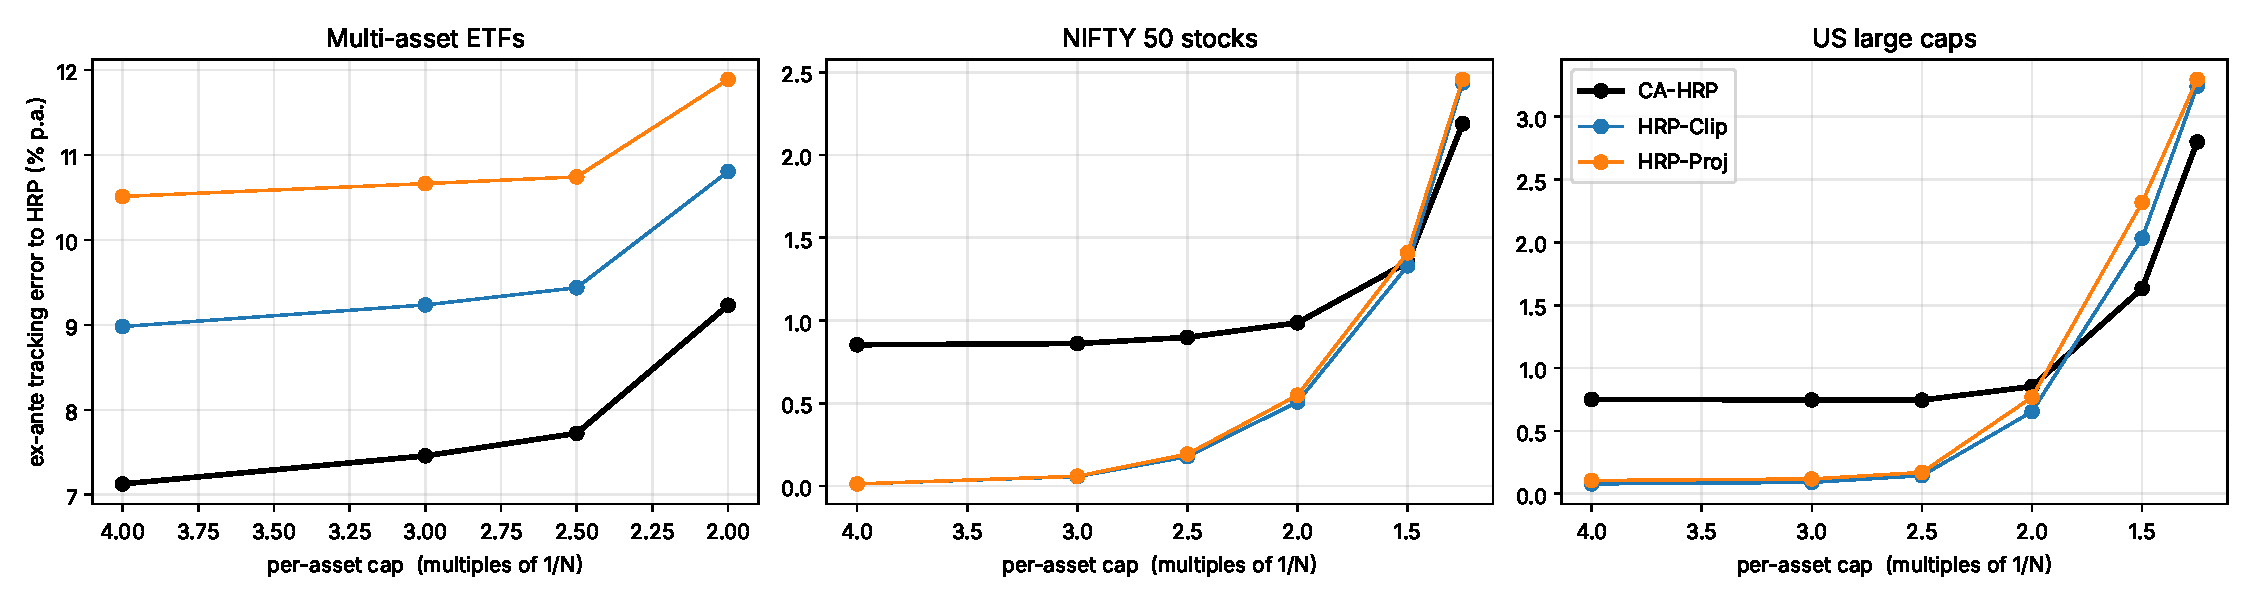
\includegraphics[width=\linewidth]{../results/figures/tightness.pdf}
\caption{Ex-ante tracking error to sample-covariance HRP as the per-asset cap tightens
(right = tighter). Infeasible settings are omitted.}
\label{fig:tight}
\end{figure}

\FloatBarrier
\section{Discussion}\label{sec:discussion}
Three lessons emerge. First, \emph{HRP is not deployable as-is} under realistic mandates:
it breaches constraints at up to every rebalance, and the clipping fix used in practice still
fails often. Second, \emph{how} constraints are enforced matters as much as \emph{whether}
they are: the same HRP target, projected with a risk-aware metric instead of a Euclidean one,
gives a portfolio with 25\% less volatility and a higher Sharpe ratio, out of sample and in
the held-out period. Third, building constraints into the bisection, while elegant and
provably feasible, is inferior to separating risk allocation from constraint enforcement.

\paragraph{Limitations.} The stock universes are survivorship-biased because they contain
current large caps; this affects all methods equally. The gains of CA-HRP are concentrated
in settings where constraints bind strongly; when they do not, it reduces to HRP, which is
by design. Most Sharpe differences are not statistically significant at conventional
levels, which is typical for portfolio comparisons over 15--20 years, and constrained
minimum variance remains a strong benchmark. Finally, the tracking-error projection
inherits the weakness of any covariance-based hedge, visible in 2022 when stock--bond
correlation turned positive.


\FloatBarrier
\section{Conclusion}\label{sec:conclusion}
We showed that Hierarchical Risk Parity, despite its robustness, cannot be used directly
under realistic portfolio mandates, and that the ad hoc fixes used in practice either fail
to restore feasibility or distort the risk allocation. Constraint-Aware HRP separates the
two problems: HRP decides how risk should be allocated, and a tracking-error projection
finds the compliant portfolio closest to that allocation in risk terms. The method has
clean theoretical properties, runs in milliseconds per rebalance, satisfied every
constraint in more than 600 rebalances across three markets, and improved risk-adjusted
returns exactly where constraints bind, including on a held-out test period. We also
proved that constraints can be embedded directly in the recursive bisection with an exact
feasibility guarantee, but found that doing so is empirically inferior, a useful negative
result for the growing literature on hierarchical allocation.

Future work includes projection metrics that adapt to regime changes in correlations, such
as the 2022 stock--bond shift, the use of CA-HRP with factor-model covariance estimates for
larger universes, and extending the capacity analysis to non-linear constraints such as
tracking-error or CVaR budgets.

\paragraph{Code and data availability.} All code, data and scripts that reproduce every
table and figure are available at \url{https://github.com/pramukhjain123/capstone}.

\bibliographystyle{plainnat}
\bibliography{refs}

\appendix
\section{Design study on the validation period}\label{app:design}
Table~\ref{tab:design} lists the eight configurations compared before the method was frozen,
using only data up to the end of the validation window. The tracking-error projection was
best in the multi-asset universe and tied for best in the stock universes. The
sample-covariance version scored marginally higher than the Ledoit--Wolf one; we kept
Ledoit--Wolf, chosen beforehand for its better conditioning, since the difference is
within noise. The initial design (``cap+tree (v0)'') was the weakest in the multi-asset
universe.

\begin{table}[h]\centering\small
\caption{Design study on the validation period only (net of 10\,bps). ``cap'' = capacity-aware bisection; ``tree'' = tree-weighted projection; ``TE'' = tracking-error projection. LW covariance unless stated.}\label{tab:design}
\begin{tabular}{l rrr rr}\toprule
 & \multicolumn{3}{c}{Validation Sharpe} & \multicolumn{2}{c}{ETFs}\\
\cmidrule(lr){2-4}\cmidrule(lr){5-6}
Variant & ETFs & NIFTY & US & Vol & Turn.\\\midrule
cap+tree (v0) & 0.605 & 1.737 & 0.639 & 10.2 & 2.59\\
euclid (LW) & 0.675 & 1.731 & 0.645 & 10.2 & 1.07\\
cap+euclid & 0.637 & 1.737 & 0.646 & 10.3 & 2.11\\
diag-var proj & 0.743 & 1.731 & 0.648 & 9.5 & 1.13\\
TE proj & 0.878 & 1.738 & 0.651 & 7.3 & 1.19\\
cap+TE proj & 0.750 & 1.737 & 0.651 & 8.6 & 2.45\\
TE+tree proj & 0.749 & 1.741 & 0.651 & 7.9 & 2.30\\
TE proj (sample cov) & 0.887 & 1.745 & 0.655 & 7.3 & 1.11\\
\bottomrule\end{tabular}\end{table}

\section{Turn-of-month returns in the NIFTY universe}
Daily returns on the last trading day of the month are unusually large in the NIFTY sample
(an average of 0.42\% for an equal-weight portfolio up to 2018, against 0.07\% on other
days). All methods trade at the month-end close and earn that day's return with their
pre-trade weights, so the effect raises all NIFTY Sharpe ratios similarly and does not
change their ranking.

\end{document}
